\documentclass{article}
\usepackage{ctex}
\usepackage{tikz}

\title{大物作业}
\author{张博涵-应化1903(学号:1912020312)}
\date{\today}

\begin{document}
	\maketitle
	\quad 由于在国际标准单位制下讨论,则在推导过程中单位进行省略.
	
	
	<1> 由题意,不妨将质点视为逆时针旋转,质点的运动至(1)所描述的位置时应是这样一种情况:
	\\
	
	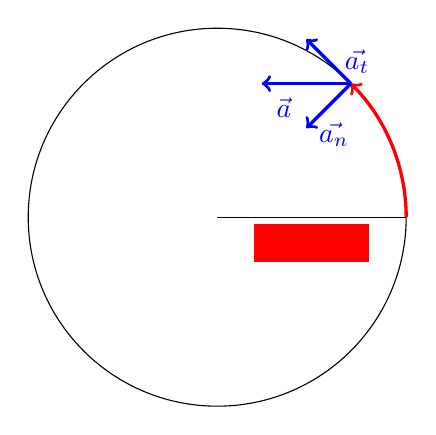
\begin{tikzpicture}[scale=0.8]
		\draw (0,0) circle (3cm);
		\draw (0,0) -- (3,0);
		\draw(0,0) -- node[below=2pt,fill=white][very thick,red] {$ R=3m $} (3,0);
        \draw[->] [very thick,red] (3cm,0) arc (0:45:3cm);
        \draw[->][very thick,blue] (1.5*1.414,1.5*1.414) --node[right=2pt,below=2pt] {$ \vec{a_n} $} (1*1.414,1*1.414);
        \draw[->][very thick,blue] (1.5*1.414,1.5*1.414) --node[right=2pt,] {$ \vec{a_t} $} (1.414,2*1.414);
        \draw[->][very thick,blue] (1.5*1.414,1.5*1.414) --node[near end,below=1pt] {$ \vec{a} $} (0.5*1.414,1.5*1.414);
	\end{tikzpicture}\\
	
	
	那么由题目所知$$\beta = \frac{d}{dt}(\frac{d\theta}{dt})=1 rad/s^2$$
	即$$d(\frac{d\theta}{dt})=dt$$
	两边积分$$\int_{0}^{t}d(\frac{d\theta}{dt})=\int_{0}^{t}dt$$
    得到$$\omega=\frac{d\theta}{dt}=t$$
    此时由向心加速度和切向加速度的公式:
    $$a_n=\omega^2R$$
    $$a_t=R\beta$$
    得
    $$a_n=3t^2,a_t=3$$
    由图可知,在总加速度方向和过此点到圆心的连线方向呈45°角时,$a_n=a_t$
    即$3=3t^2$由于$t>0$则解得$t=1s$
    
    <2>已知$\omega$
    则可得到$v=R\omega=3t$即$$\frac{ds}{dt}=3t$$
    移项积分:
    $$\int_{0}^{t}dr=\int_{0}^{t}3tdt$$
    即$s=1.5t^2$
    此时$t=1s$带入可解得$s=1.5m$
    
    答: \quad (1)$t=1s$ \quad (2)$s=1.5m$
    
	
\end{document}